\documentclass[11pt]{article}
% DEFINE COMMANDS

\usepackage{NotesTeX}

\usepackage[font=small,labelfont=bf]{caption}
\usepackage{enumerate}
\usepackage{amsmath,amssymb,amscd,amsfonts}
\usepackage{xcolor}
\usepackage{color}


\usepackage{tikz}
\usepackage{tikz-cd}
\tikzcdset{every label/.append style = {font = \small}}
\tikzcdset{row sep/normal=3.5em}
\tikzcdset{column sep/normal=3.5em}

\usetikzlibrary{matrix}
\usetikzlibrary{decorations.markings,calc,shapes}
\usetikzlibrary{positioning}
\usepackage{graphicx}
\usepackage{empheq}
\usepackage{physics}
\usepackage{siunitx}
\usepackage{tensor}

\usepackage{multicol}

\usepackage{youngtab}
\usepackage{cancel}
\usepackage{caption}
\usepackage{graphicx}
\usepackage{subcaption}
\usepackage{hyperref}

\usepackage{float}
\makeatletter
\RenewDocumentCommand\sidenotetext{ o o +m }{%      
    \IfNoValueOrEmptyTF{#1}{%
        \@sidenotes@placemarginal{#2}{\textsuperscript{\thesidenote}{}~\footnotesize#3}%
        \refstepcounter{sidenote}%
    }{%
        \@sidenotes@placemarginal{#2}{\textsuperscript{#1}~#3}%
    }%
}
\makeatother
% % % % % % % % % % % % % % % % % % % % % % %

\title{{\Huge General Relativity}\\{\Large{Class 1 --- January 22, 2020}}} %replace with class number
\author{Sanjit Shashi}

\emailAdd{sshashi@utexas.edu} %replace with your email
\begin{document}
\maketitle
\flushbottom
\newpage
\pagestyle{fancynotes}

\part{Introduction}
\section{Geometric Viewpoints}

It is nice to make equations describing the physical world as \textbf{invariant} as possible. This is why we like geometric representations of physical systems; they are independent of things like coordinate transformations. For example, recall Newton's second law,
\begin{equation}
\textbf{F} = \frac{d\textbf{p}}{dt}\ .\label{newton}
\end{equation}

The vectors $\textbf{p}$ and $\textbf{F}$ are geometrical objects which always satisfy (\ref{newton}) without any regard to a variety of coordinate transformations. For example, consider \textbf{rotation} (in this case, about the $z$ axis).
\begin{figure}[H]    
\centering
\begin{tikzpicture}
\draw[->] (-0.5,0,0) to (2.5,0,0);
\draw[->] (0,-0.5,0) to (0,2.5,0);
\draw[->] (0,0,-0.5) to (0,0,2.5);
\node at (2.5,-0.3) {$x$};
\node at (-0.3,2.5) {$y$};
\node at (-0.3,0,2.5) {$z$};
\draw[->,very thick] (0,0,0) to (1.5,1.5,0);
\node at (1.3,1.8,0) {$\textbf{F}$};
\draw[-,dashed] (1.5,1.5) to (1.5,-0.5) to (0,0);
\end{tikzpicture}
\begin{tikzpicture}
\node at (0,0) {$\implies$};
\node at (0,-2) {};
\end{tikzpicture}
\begin{tikzpicture}
\draw[->,rotate=30] (-0.5,0,0) to (2.5,0,0);
\draw[->,rotate=30] (0,-0.5,0) to (0,2.5,0);
\draw[->] (0,0,-0.5) to (0,0,2.5);
\node at (2.5,1) {$x'$};
\node at (-1.3,2.3) {$y'$};
\node at (-0.3,0,2.5) {$z'$};
\draw[->,very thick] (0,0,0) to (1.5,1.5,0);
\node at (1.3,1.8,0) {$\textbf{F}$};
\draw[-,dashed] (1.5,1.5) to (2,0.5) to (0,0);
\end{tikzpicture}
\caption{}
\end{figure}

The actual vector $\textbf{F}$ does not change; it is invariant under rotation.\footnote{We will discuss later, however, that the vector's $x'$, $y'$, and $z'$ components are not the same as the $x$, $y$, and $z$ components.}

Equation (\ref{newton}) is also invariant under a \textbf{Galilean boost}, in which we go, for example, from $(x,y,z)$ to $(x',y',z')$ by,
\begin{align}
x' &= x-Vt\ ,\\
y' &= y\ ,\\
z' &= z\ ,
\end{align}
where $V$ is some speed.\pagebreak

Pictorially, the $(x',y',z')$ coordinate system is moving with respect to the $(x,y,z)$ coordinate system (in this case, along the $x$ direction).

\begin{figure}[H]    
\centering
\begin{tikzpicture}
\draw[->] (-0.5,0,0) to (2.5,0,0);
\draw[->] (0,-0.5,0) to (0,2.5,0);
\draw[->] (0,0,-0.5) to (0,0,2.5);
\node at (2.5,-0.3) {$x$};
\node at (-0.3,2.5) {$y$};
\node at (-0.3,0,2.5) {$z$};
\draw[->,very thick] (0,0,0) to (1.5,1.5,0);
\node at (1.3,1.8,0) {$\textbf{F}$};
\draw[-,dashed] (1.5,1.5) to (1.5,-0.5) to (0,0);
\end{tikzpicture}
\begin{tikzpicture}
\draw[->] (-0.5,0,0) to (2.5,0,0);
\draw[->] (0,-0.5,0) to (0,2.5,0);
\draw[->] (0,0,-0.5) to (0,0,2.5);
\node at (2.5,-0.3) {$x'$};
\node at (-0.3,2.5) {$y'$};
\node at (-0.3,0,2.5) {$z'$};
\draw[->] (1,1) to (2,1);
\node at (1.5,1.3) {$V$};
\end{tikzpicture}
\caption{}
\end{figure}

More generally, we can write a Galilean transformation from $\textbf{r} = (x,y,z)$ to $\textbf{r}' = (x',y',z')$ with corresponding velocity $\textbf{V}$ in terms of the velocities of the two systems $\textbf{u} = \dot{\textbf{r}}$ and $\textbf{u}' = \dot{\textbf{r}}'$,
\begin{equation}
\textbf{u}' = \textbf{u} - \textbf{V}\ .
\end{equation}

The coordinate systems in which (\ref{newton}) holds for the geometrical objects $\textbf{F}$ and $\textbf{p}$ are called \textbf{inertial frames}.

We need to distinguish the geometrical objects (such as the vectors above, or, even more generally, tensors) from their \textbf{(coordinate-dependent) components}. For example, with $\textbf{F}$, we have that,
\begin{equation}
\textbf{F} = \sum_{i=1}^3 F^i \textbf{e}_{(i)}\ .
\end{equation}

The vectors $\textbf{e}_{(i)}$ are \textbf{basis vectors}. In Cartesian coordinates, we write,
\begin{align}
\textbf{e}_{(1)} &= \hat{\textbf{x}}\ ,\\
\textbf{e}_{(2)} &= \hat{\textbf{y}}\ ,\\
\textbf{e}_{(3)} &= \hat{\textbf{z}}\ .
\end{align}
Meanwhile, the $F^i$ are the \textbf{components}.

Relating this to the above discussion about coordinate transformations, we can consider how rotation (specifically about the $z$-axis again) transforms the components of $\textbf{F}$. The transformation is,
\begin{equation}
F^{i'} = \sum_{j=1}^3 \tensor{R}{^{i'}_{j}} F^j\ \ \ \left(\tensor{R}{^{i'}_{j}} = \begin{pmatrix}
\cos\theta& \sin\theta & 0\\
-\sin\theta & \cos\theta & 0\\
0 & 0 & 1\\
\end{pmatrix}\right)\ .\label{sumComp}
\end{equation}
Again, pictorially, the $x$, $y$, $x'$, and $y'$ components\footnote{We suppress the $z$ direction because we are rotating around it, so $F^3 = F^{3'}$.} of $\textbf{F}$ are,

\begin{figure}[H]    
\centering
\begin{tikzpicture}
\draw[->,color=blue] (-0.5,0,0) to (2.5,0,0);
\draw[->,color=blue] (0,-0.5,0) to (0,2.5,0);
\node at (2.5,-0.3) {$x$};
\node at (-0.3,2.5) {$y$};
\draw[->,rotate=30,color=red] (-0.5,0,0) to (2.5,0,0);
\draw[->,rotate=30,color=red] (0,-0.5,0) to (0,2.5,0);
\node at (2.5,1) {$x'$};
\node at (-1.3,2.3) {$y'$};
\draw[-,dashed,color=blue] (1.5,1.5) to (0,1.5);
\draw[-,dashed,color=blue] (1.5,1.5) to (1.5,0);
\node at (-0.3,1.5) {$F^2$};
\node at (1.5,-0.3) {$F^1$};
\draw[-,dashed,color=red] (1.5,1.5) to (-0.27,0.47);
\draw[-,dashed,color=red] (1.5,1.5) to (1.77,1.02);
\node at (1.87,0.82) {$F^{1'}$};
\node at (-0.6,0.32) {$F^{2'}$};
\draw[->,very thick] (0,0,0) to (1.5,1.5,0);
\node at (1.3,1.8,0) {$\textbf{F}$};
\end{tikzpicture}
\caption{}
\end{figure}


Also, we can write the sum in (\ref{sumComp}) in matrix notation,
\[
\begin{pmatrix}
F^{1'}\\
F^{2'}\\
F^{3'}
\end{pmatrix} = \begin{pmatrix}
\cos\theta& \sin\theta & 0\\
-\sin\theta & \cos\theta & 0\\
0 & 0 & 1\\
\end{pmatrix}\begin{pmatrix}
F^1\\
F^2\\
F^3
\end{pmatrix}
\]
But, working with matrices can be more annoying algebraically, because we do not have commutativity. This is the upshot of working in the summation notation.

However, transforming the components becomes more unwieldy when we consider objects besides vectors with more indices. A larger number of indices means that we need to use more matrices; in the summation notation, this means that we have larger sums with more terms. So, using sums quickly becomes inconvenient.

\section{Einstein Notation}

\textbf{Einstein notation} (also called \textbf{Einstein summation convention}) is a very convenient shorthand for sums. For example, (\ref{sumComp}) would be written as,
\begin{equation}
F^{i'} = R^{i'}_{j} F^j\ ,
\end{equation}
\textit{i.e.} we drop the $\Sigma$ symbol and implicitly sum over the $j$ index.\\

When we use Einstein notation, the position of the indices on an expression matters. In particular,
\begin{equation}
R_{i'j} \neq \tensor{R}{^{i'}_j}\ ;\ F^{i'} \neq F_{i'}\ (\text{in general})\ .
\end{equation}

In Einstein notation, there are two types of indices: \textbf{free indices} and \textbf{dummy indices}. For example, say we have an expression,
\begin{equation}
A^i = T^{ij} n_j\ .
\end{equation}

So, we are summing over the $j$ index, but the $i$ index is just floating there and must be present on both sides of the equation. Dummy indices (like $j$) are \textbf{always} summed over; convention dictates that they always come in pairs, with one being \textbf{raised} (written as a superscript) and one being \textbf{lowered} (written as a subscript).\sidenote[][-9\baselineskip]{Choice of alphabet does not matter for repeated indices because they do not appear in the sum evaluated. This means that we can write something like,
\begin{equation}
T^{ij}n_j = T^{ik}n_k\ .
\end{equation}
However, we must always be sure to obey the above rules of dummy indices coming in pairs and free indices being alone.
}

Meanwhile, free indices (like $i$) must be alone and must appear on both sides.\\



\part{Special Relativity}

\section{Motivation}

The core principle of relativity is that physics should be the same for \textbf{all} inertial observers. However, Maxwell's equations created a problem; they gave us the speed of light $c$.\\

There is a lot of depth to the story of how the speed of light was problematic (see Michelson-Morley as a particularly important experiment), but, essentially, $c$ is always observed to be at its particular value in all inertial frames, even under Galilean boosts. This is where special relativity enters the picture; it is meant to give us an arena in which we account for this quirk of $c$.

\section{Spacetime}

The idea is to treat time as another dimension, so, instead of space, we think about \textbf{spacetime}. Points in spacetime (called \textbf{events}) are labeled by $(x^0,x^1,x^2,x^3)$ (or, using Cartesian coordinates again, $(x^0,x,y,z)$), where,
\begin{equation}
x^0 = ct\ .
\end{equation}

In SI, we multiply $t$ by $c$ to get units of distance. However, from now on, we will use units in which $c = 1$, which just means that time is measured in units of distance while velocity becomes \textbf{dimensionless}.

Before, we used Latin indices ($i$, $j$, etc.) to denote the components of vectors and tensors in space. To denote components in spacetime, we use \textbf{Greek indices} ($\mu$, $\nu$, etc.). While Latin indices are always taken to run from $1$ to $3$, Greek indices are supposed to run from $0$ to $3$. For example,
\begin{equation}
x^\mu = \begin{pmatrix}
x^0\\
x^1\\
x^2\\
x^3
\end{pmatrix} = \begin{pmatrix}
t\\
x\\
y\\
z
\end{pmatrix}\ .
\end{equation}

To make our lives easier, we will often rotate our coordinates so that everything is happening on the $tx$-axis. This way, we can suppress the $y$ and $z$ axes when talking about SR.

The path followed by an observer through spacetime is called its \textbf{worldline}. Meanwhile, the path followed by something moving at $c$ (such as a photon) is called a \textbf{light ray}. To get a better idea of what these are, consider the following \textbf{spacetime diagram}, which is essentially just a $t$ vs. $x$ plot.

\begin{figure}[H]    
\centering
\begin{tikzpicture}
\draw[->] (0,-1) to (0,2.5);
\draw[->] (-2.5,0) to (2.5,0);
\draw[-,very thick,color=blue] (0,-0.5) to (0,2);
\draw[-,thick,color=green] (-0.25,-0.5) to (1,2);
\draw[-,thick,color=green] (0,0) to (1,2);
\draw[-,thick,color=purple] (0.25,-0.5) .. controls (0,-0.4) .. (0,0) .. controls (-0.5,1.5) .. (-1.8,2);
\draw[-] (1,0) arc (0:45:1);
\node at (1.3,0.3) {$45^\circ$};
\draw[-] (-1,0) arc (180:135:1);
\node at (-1.3,0.3) {$45^\circ$};
\draw[-,very thick,dashed,color=red] (-0.5,-0.5) to (2.5,2.5);
\draw[-,very thick,dashed,color=red] (0.5,-0.5) to (-2.5,2.5);
\node at (0,0) {$\bullet$};
\node at (2.5,-0.3) {$x$};
\node at (0.3,2.5) {$t$};
\end{tikzpicture}
\caption{}
\end{figure}

Spacetime diagrams can be thought of as corresponding to some observer who remains at the spatial origin; above, the blue line is the worldline of such an observer.

Furthermore, anything which has a worldline that is straight has a constant speed, which is given by the reciprocal of the slope. The blue worldline corresponds to a speed of $0$, while the green worldline corresponds to a speed less than $1$ (\textit{i.e.} less than $c$). The purple line has a non-constant speed.

What about the red lines? Those are the light rays which are emanating from the origin; they have slopes of $\pm 1$, so they correspond to objects moving at speed $c$ along the $\pm x$ direction. At each event in spacetime, the light rays which emanate from that particular event define a \textbf{light cone}. Photons and other massless particles which move at $c$ will always move along the surface of a light cone, while massive particles move \textbf{within} the lightcones. Massive particles can never leave a light cone.

\begin{figure}[H]    
\centering
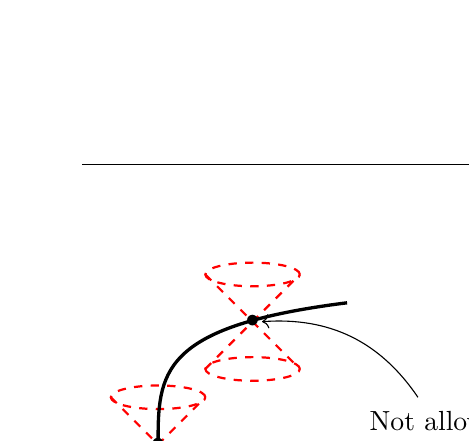
\begin{tikzpicture}[scale=0.6]
\draw[-,color=red,dashed,thick] (-1,-1) to (1,1);
\draw[-,color=red,dashed,thick] (-1,1) to (1,-1);
\draw[-,color=red,dashed,thick] (0,1) ellipse (1 and 0.25);
\draw[-,color=red,dashed,thick] (0,-1) ellipse (1 and 0.25);
\node at (0,0) {$\bullet$};
\draw[-,color=red,dashed,thick] (-1,-1+3) to (1,1+3);
\draw[-,color=red,dashed,thick] (-1,1+3) to (1,-1+3);
\draw[-,color=red,dashed,thick] (0,1+3) ellipse (1 and 0.25);
\draw[-,color=red,dashed,thick] (0,-1+3) ellipse (1 and 0.25);
\node at (0,3) {$\bullet$};
\draw[-,color=red,dashed,thick] (-1+2,-1+5.6) to (1+2,1+5.6);
\draw[-,color=red,dashed,thick] (-1+2,1+5.6) to (1+2,-1+5.6);
\draw[-,color=red,dashed,thick] (0+2,1+5.6) ellipse (1 and 0.25);
\draw[-,color=red,dashed,thick] (0+2,-1+5.6) ellipse (1 and 0.25);
\node at (0+2,3+2.6) {$\bullet$};
\draw[-,very thick] (-0.5,-1) .. controls (0,-0.3) .. (0,0) .. controls (0.5,1.5) .. (0,3) .. controls (0,4.5) and (0,5.5) .. (4,6);
\node at (6,3.5) {Not allowed};
\node at (6,2.75) {for particles};
\draw[->] (5.5,4) to[bend right] (2.2,5.6);
\end{tikzpicture}
\caption{}
\end{figure}    
 
\end{document}
